% !TEX encoding = UTF-8 Unicode
% -*- coding: UTF-8; -*-
\ifdefined\ishandout
\documentclass[handout]{beamer}
\else
\documentclass[11pt]{beamer}
\fi

\usepackage[frenchb]{babel}
\usepackage[T1]{fontenc}
\usepackage[utf8]{inputenc}
\usepackage{hyperref}
\usepackage{multirow}
\usepackage{listings}
\usepackage{fancyvrb}
\usepackage{tikz}
\usepackage{framed}
\usepackage{algorithm}
\usepackage{algorithmic}
\usepackage{xcolor}
\usepackage{color, colortbl}
\ifdefined\ishandout
\usepackage{handoutWithNotes}
\fi
\usepackage{slashbox}
\usepackage{amsmath}
\usepackage{bm}
\usepackage{hhline}
\usepackage{xmpmulti}
\usepackage{pgfplots}

\usetikzlibrary{shapes.geometric}
\usetikzlibrary{positioning}
\usetikzlibrary{shapes.arrows, chains}
\usetikzlibrary{arrows,calc}
\usetikzlibrary{shapes.multipart}
\usepackage{array}
\usetheme{Boadilla}

\usefonttheme[onlymath]{serif}

\newcommand{\R}{\mathbb{R}}
\newcommand{\C}{\mathbb{C}}
\newcommand{\N}{\mathbb{N}}
\newcommand{\Z}{\mathbb{Z}}
\newcommand{\E}{\mathbb{E}}
\newcommand{\Var}{\text{Var}}
\newcommand{\Cov}{\text{Cov}}
\ifdefined\ishandout
\pgfpagesuselayout{3 on 1 with notes}[a4paper,border shrink=5mm]
\usecolortheme{dove}
\else
%\usecolortheme{dolphin}
\usecolortheme{beaver}
\fi


\lstnewenvironment{codeC}
{ \lstset{language=C,
    otherkeywords={printf,scanf}}
}
{}

\ifdefined\ishandout
\definecolor{mygreen}{rgb}{0,0,0}
\definecolor{mymauve}{rgb}{0,0,0}
\definecolor{myblue}{rgb}{0,0,0}
\else
\definecolor{mygreen}{rgb}{0,0.6,0}
\definecolor{mymauve}{rgb}{0.58,0,0.82}
\definecolor{myblue}{rgb}{0,0,1}

\fi

%% Notes
%\setbeameroption{show only notes}


\definecolor{mygray}{rgb}{0.5,0.5,0.5}

\lstset{ language=Python,%
  backgroundcolor=\color{white},   % choose the background color; you must add \usepackage{color} or \usepackage{xcolor}
  basicstyle=\footnotesize,        % the size of the fonts that are used for the code
  breakatwhitespace=false,         % sets if automatic breaks should only happen at whitespace
  breaklines=true,                 % sets automatic line breaking
  captionpos=b,                    % sets the caption-position to bottom
  commentstyle=\color{mygreen},    % comment style
  deletekeywords={...},            % if you want to delete keywords from the given language
  escapeinside={\%*}{*)},          % if you want to add LaTeX within your code
  extendedchars=true,              % lets you use non-ASCII characters; for 8-bits encodings only, does not work with UTF-8
  frame=tb,	                   % adds a frame around the code
  keepspaces=true,                 % keeps spaces in text, useful for keeping indentation of code (possibly needs columns=flexible)
  keywordstyle=\color{blue},       % keyword style
  otherkeywords={*,...},           % if you want to add more keywords to the set
  numbers=none,                    % where to put the line-numbers; possible values are (none, left, right)
  numbersep=5pt,                   % how far the line-numbers are from the code
  numberstyle=\tiny\color{mygray}, % the style that is used for the line-numbers
  rulecolor=\color{black},         % if not set, the frame-color may be changed on line-breaks within not-black text (e.g. comments (green here))
  showspaces=false,                % show spaces everywhere adding particular underscores; it overrides 'showstringspaces'
  showstringspaces=false,          % underline spaces within strings only
  showtabs=false,                  % show tabs within strings adding particular underscores
  stepnumber=2,                    % the step between two line-numbers. If it's 1, each line will be numbered
  stringstyle=\color{mymauve},     % string literal style
  tabsize=3,	                   % sets default tabsize to 2 spaces
  title=\lstname                   % show the filename of files included with \lstinputlisting; also try caption instead of title
}
%\lstset{language=Python,
% breakatwhitespace=false,         % sets if automatic breaks should only happen at whitespace
%  breaklines=true,                 % sets automatic line breaking
%  captionpos=b,                
%%commentstyle=\itshape\color{mymauve},
%%keywordstyle=\bfseries\color{myblue},
%numbers=left,                    % where to put the line-numbers; possible values are (none, left, right)
%  numbersep=8pt,                   % how far the line-numbers are from the code
%  numberstyle=\tiny\color{mygray}, % the style that is used for the line-numbers
%%  rulecolor=\color{black},         % if not set, the frame-color may be changed on line-breaks within not-black text (e.g. comments (green here))
%  showspaces=false,                % show spaces everywhere adding particular underscores; it overrides 'showstringspaces'
%%  showstringspaces=false,          % underline spaces within strings only
%  showtabs=false,                  % show tabs within strings adding particular underscores
%  stepnumber=2,                    % the step between two line-numbers. If it's 1, each line will be numbered
%%  stringstyle=\color{mygreen},     % string literal style
%  tabsize=2 
%}
\ifdefined\ishandout
\newcommand{\red}{\textbf}
\else
\newcommand{\red}{\textcolor{red}}
\fi
%\newcommand \emph
%Default size : 12.8 cm * 9.6 cm

\newcommand{\tmark}[1]{\tikz[remember picture, baseline=-.5ex]{\coordinate(#1);}}

\ifdefined\ishandout
\newenvironment<>{codeblock}[1]{%begin
  \setbeamercolor{block title}{fg=black,bg=lightgray!80}%
  \begin{block}{#1}}
  % \begin{codeC}}
  %  {\end{codeC}
{  
\end{block}}

\newenvironment<>{termblock}[1]{
    \setbeamercolor{block title}{fg=black,bg=lightgray!90}%
    \begin{block}{#1}
}
%     \begin{Verbatim}}
{%\end{Verbatim}
\end{block}
}

\definecolor{bluegreen}{RGB}{0,0,0}
%\definecolor{bluegreen}{rgb}{0,0.6,0.8}
\else

\newenvironment<>{codeblock}[1]{%begin
  \setbeamercolor{block title}{fg=darkgray,bg=yellow}%
  \begin{block}{#1}}
  % \begin{codeC}}
  %  {\end{codeC}
{  
\end{block}}

\newenvironment<>{termblock}[1]{
    \setbeamercolor{block title}{fg=white,bg=lightgray}%
    \begin{block}{#1}}
%     \begin{Verbatim}}
{%\end{Verbatim}
\end{block}
}

\definecolor{bluegreen}{RGB}{0,149,182}
%\definecolor{bluegreen}{rgb}{0,0.6,0.8}
\fi

%\newcommand{\output}[1]{
\setbeamertemplate{navigation symbols}{}
\newcommand{\bvrb}{\Verb[commandchars=£µ§,formatcom=\color{bluegreen}]}
\newcommand{\footvrb}{\footnotesize\Verb}
\newcommand{\vrbalert}[2][]{\visible<#1>{#2}}
%%% Commande pour les listes/arbres
\newcommand{\mvide}{\nodepart{one} \nodepart{two}}
\newcommand{\tvide}{\nodepart{one} \nodepart{two} \nodepart{three}}
\newcommand{\rref}[1][]{\hfill{\scriptsize\textit{#1}}}


\newcommand{\odif}[2]{\frac{d #1}{d #2}} 
%%Fin des commandes pour les listes/arbres.
\newcommand{\gooditem}[1]{\setbeamercolor{item}{fg=green}\item #1} 
\newcommand{\pooritem}[1]{\setbeamercolor{item}{fg=red}\item #1} 
\setbeamerfont{caption}{size=\scriptsize}

%%% Paramètres du cours (à régler)
%Numéro du cours
\newcommand{\nb}{1}

\title[machine learning]{Machine Learning à l'IPSL}
\author[J. Brajard]{julien.brajard@sorbonne-universite.fr}
\institute[LOCEAN/SU]{LOCEAN-SU}
\date{13 Mars 2018}
\begin{document}
\tikzstyle{every picture}+=[remember picture]
%%%%%%%%%%%%%%%%%%%%% SLIDES DE TITRE
\begin{frame}
\titlepage
%\centering{
%\url{http://australe.upmc.fr} (onglet EPU-C5-IGE Info Gen)}
\end{frame}

%%%%%%%%%%%%%%%%%%%%
\begin{frame}
\frametitle{What is machine learning ?}
\begin{block}{A machine}
\begin{equation*}
y = \mathcal{M}(x,\theta)
\end{equation*}
\begin{itemize}
\item $x$: input
\item $y$: output
\item $\mathcal{M}$: a model (named "machine")
\item $\theta$ : parameters of the model $\mathcal{M}$.
\end{itemize}
\end{block}
\alert{Machine learning} consists in optimizing $\theta$ using a set of data. 
This is the training process.
\end{frame}



%%%%%%%%%%%%%%%%%%%%
\begin{frame}
\frametitle{Example 1: Computer Vision}
\begin{figure}
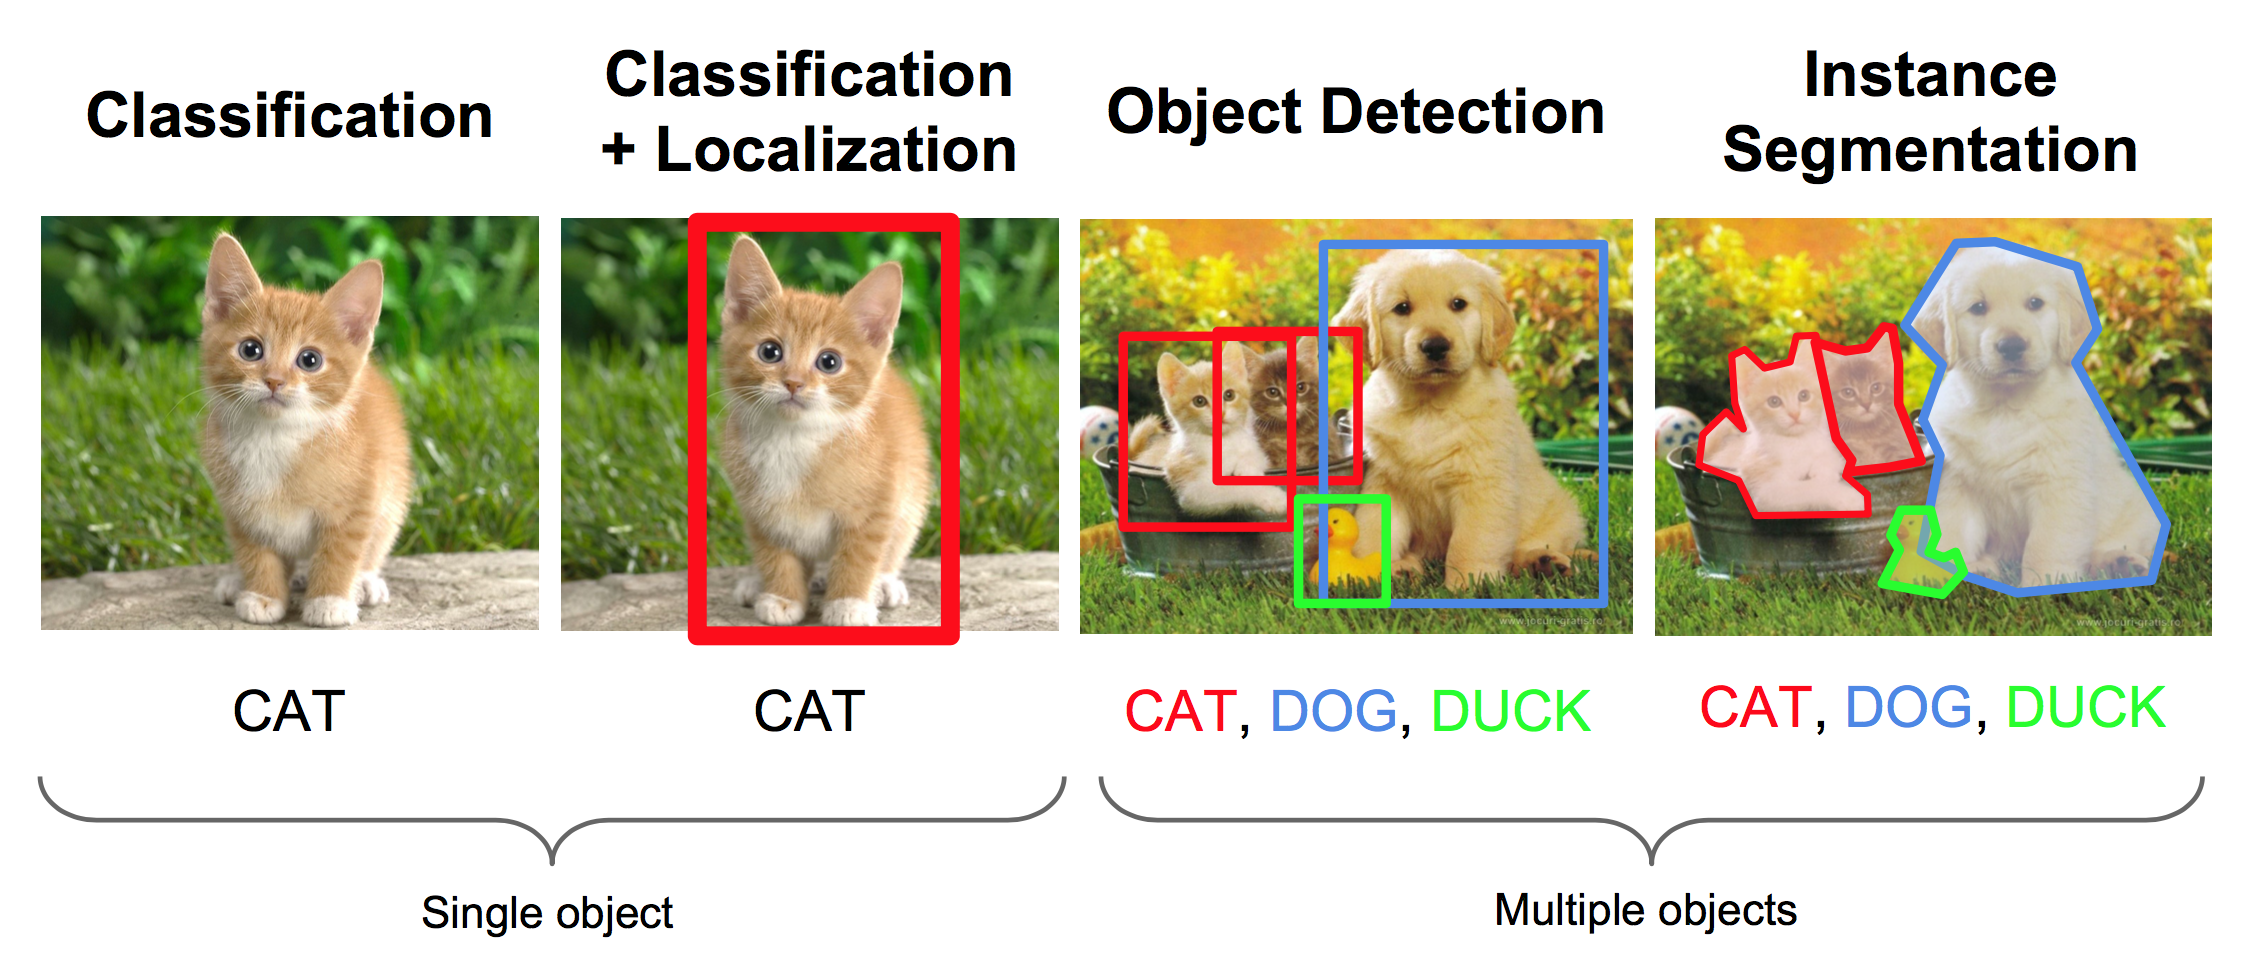
\includegraphics[width=\textwidth]{./figs/compute-vision.png}
\end{figure}
\rref[Li, Karpathy and Johnson, 2016, Stanford CS231n course]

\end{frame}


%%%%%%%%%%%%%%%%%%%%
\begin{frame}
\frametitle{Example 1: Computer Vision}
\framesubtitle{Image Net Large Scale Recogonition Challenge (ILSVRC)}
\begin{figure}

\begin{tikzpicture} [scale=0.8, every node/.style={scale=0.6}]
  \begin{axis}[ 
    x tick label style={ 
      /pgf/number format/1000 sep=}, 
    ylabel=Classification error, 
    xtick={2010,2011,2012,2013,2014,2015,2016,2017},
    xticklabels={2010,2011,2012,2013,2014,2015,2016,hum.},
    enlargelimits=0.15, 
     bar width=7pt, 
    ybar,
   legend style={at={(0.5,-0.15)},
     anchor=north,legend columns=-1}, 
   x tick label style={font=\footnotesize,rotate=45, anchor=east},
   very axis plot/.append style={
      ybar,
      bar width=.2,
      bar shift=0pt,
      fill},
      nodes near coords,
   ] 
   \addplot[ybar,fill=blue!60, bar shift=0pt]
   coordinates {(2010,28) (2011,26)}; 
   \addplot[ybar,fill=red!60]
   coordinates {(2012,16) (2013,12) (2014,7) (2015,3.6) (2016,3)}; 
   \addplot[ybar,fill=green!60, bar shift=0pt] 
   coordinates 
   {(2017,5.1)};  
   \legend{traditional algo.,Deep Learning,Human}
 \end{axis} 
\end{tikzpicture}
\end{figure}
Deep learning architectures was based on Convolutional Neural Networks (CNN).
\end{frame}



%%%%%%%%%%%%%%%%%%%%
\begin{frame}
\frametitle{Machine Translation}
Objective : translate a text from a language to another.
\begin{figure}

\includegraphics[width=.6\textwidth]{./figs/google-trad.png}
\end{figure}
\begin{itemize}
\item 2014: First scientic paper in neural networks in machine translation.
\item 2016: Neural machine translation outperform tradiational approaches on public benchmarks
\item 2017: Most of the systems (Google, Systran, WIPO) switch to
  neural machine translation  (using recurrent neural networks)
\end{itemize}
\end{frame}


%%%%%%%%%%%%%%%%%%%%
\begin{frame}
\frametitle{Advances in machine learning}
\framesubtitle{Example 2: Playing games}
\begin{columns}
\column{.5\textwidth}
\begin{itemize}
\item 1997: Deep Blue defeats Kasparov at Chess.
\item 2016: AlphaGo's victory again Lee Sedol at Go.
\item 2017: AphaGo Zero learns how to play Go only by playing against
  itself. It outperformed previous AlphaGo version (Reinforcement
  learning)
\item 2017: DeepStack beats professional human poker players.
\end{itemize}
\column{.5\textwidth}
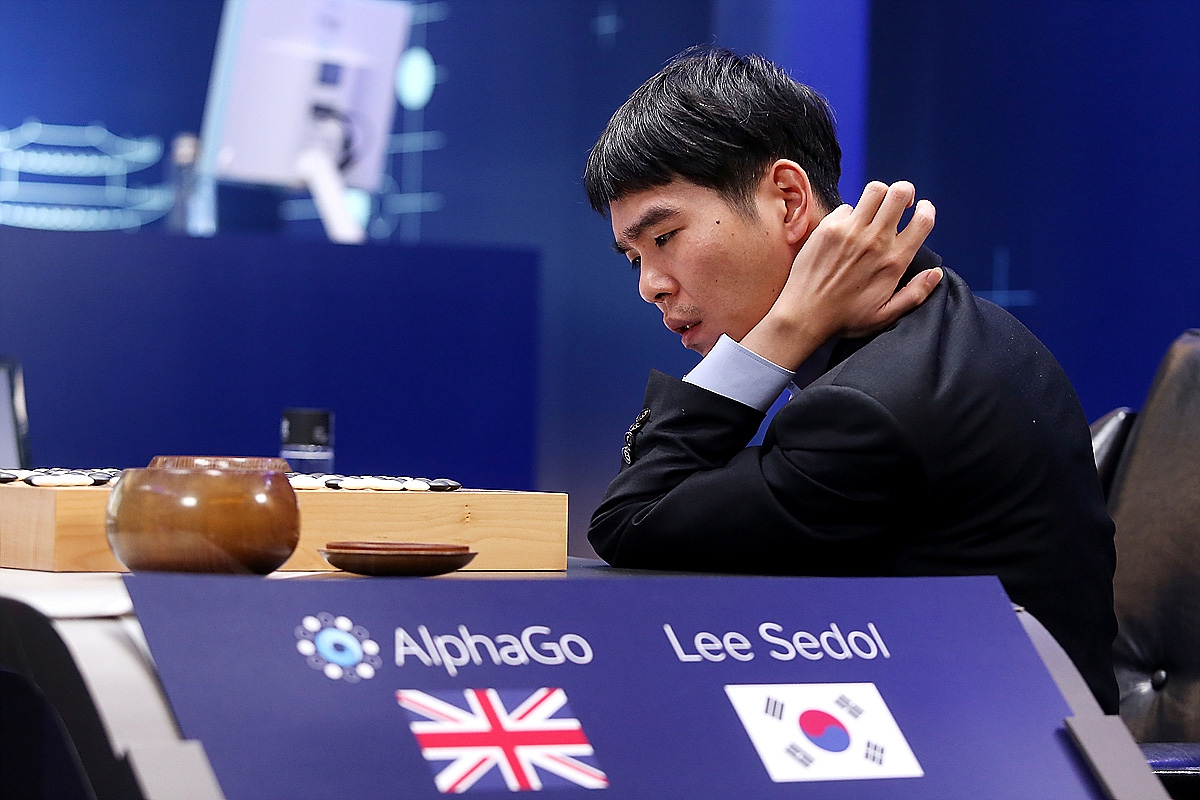
\includegraphics[width=\textwidth]{./figs/alphago.jpg}
\end{columns}
\end{frame}

%%%%%%%%%%%%%%%%%%%%
\begin{frame}
\frametitle{Link between climate-related study and machine learning }
\begin{figure}
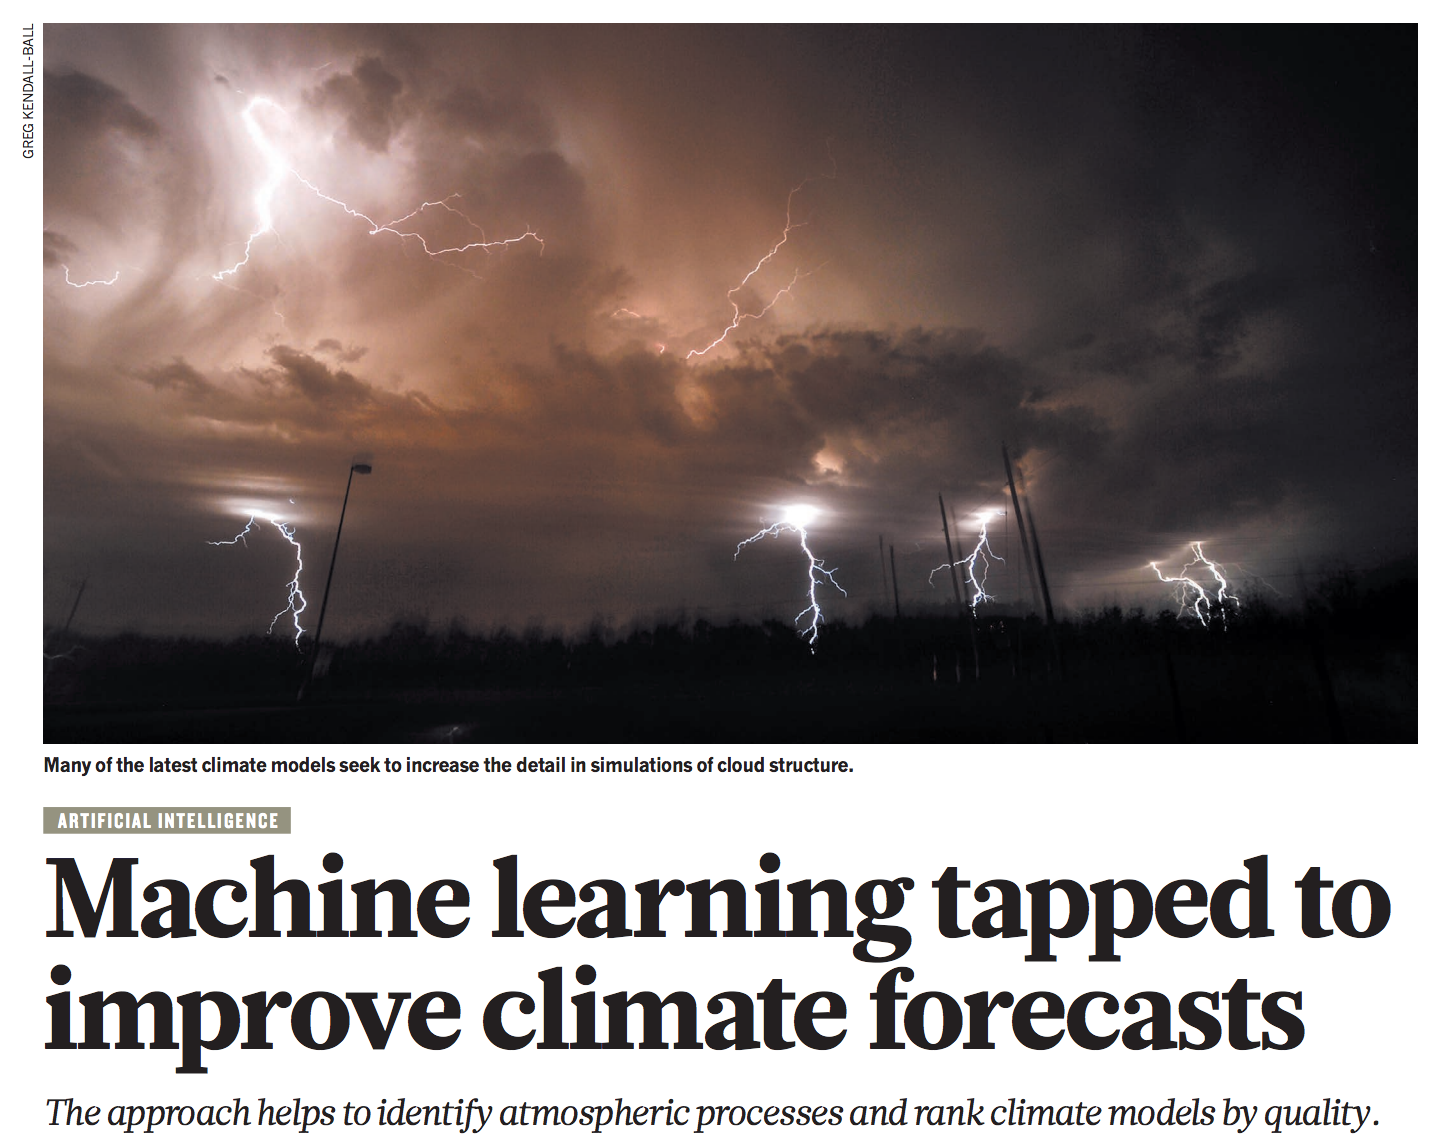
\includegraphics[height=.7\textheight]{./figs/nature.png}
\rref{Jones, Nature 548, 379–380 (24 August 2017)}
\end{figure}
\end{frame}


%%%%%%%%%%%%%%%%%%%%
\begin{frame}
\frametitle{Subjects to be addressed}
Forecasts
Nowcast
Feature identification
parameter estimation
quality control
model aggregation
\end{frame}

%%%%%%%%%%%%%%%%%%%%
\begin{frame}
\frametitle{Some examples}
Inpainting
parametrization
climate thiria


\end{frame}
%%%%%%%%%%%%%%%%%%%%
\begin{frame}
\frametitle{Some examples}
Inpainting
parametrization
climate


\end{frame}
\end{document}